\documentclass[12pt]{article}

\newcommand{\CiteMathPackage}{../Notes/math}
\newcommand{\CiteReference}{../Notes/reference.bib}

% Packages
\usepackage{setspace,geometry,fancyvrb,rotating}
\usepackage{marginnote,datetime,enumitem}
\usepackage{titlesec,indentfirst}
\usepackage{amsmath,amsfonts,amssymb,amsthm,mathtools}
\usepackage{threeparttable,booktabs,adjustbox}
\usepackage{graphicx,epstopdf,float,soul,subfig}
\usepackage[toc,page]{appendix}
\usdate

% Page Setup
\geometry{scale=0.8}
\titleformat{\paragraph}[runin]{\itshape}{}{}{}[.]
\titlelabel{\thetitle.\;}
\setlength{\parindent}{10pt}
\setlength{\parskip}{10pt}
\usepackage{Alegreya}
\usepackage[T1]{fontenc}

%% Bibliography
\usepackage{natbib,fancybox,url,xcolor}
\definecolor{MyBlue}{rgb}{0,0.2,0.6}
\definecolor{MyRed}{rgb}{0.4,0,0.1}
\definecolor{MyGreen}{rgb}{0,0.4,0}
\definecolor{MyPink}{HTML}{E50379}
\newcommand{\highlightR}[1]{{\emph{\color{MyRed}{#1}}}} 
\newcommand{\highlightB}[1]{{\emph{\color{MyBlue}{#1}}}}
\newcommand{\highlightP}[1]{{\emph{\color{MyPink}{#1}}}}
\usepackage[bookmarks=true,bookmarksnumbered=true,colorlinks=true,linkcolor=MyBlue,citecolor=MyRed,filecolor=MyBlue,urlcolor=MyGreen]{hyperref}
\bibliographystyle{econ}

%% Theorem Environment
\theoremstyle{definition}
\newtheorem{assumption}{Assumption}
\newtheorem{definition}{Definition}
\newtheorem{theorem}{Theorem}
\newtheorem{proposition}{Proposition}
\newtheorem{lemma}[theorem]{Lemma}
\newtheorem{example}[theorem]{Example}
\newtheorem{corollary}[theorem]{Corollary}
\usepackage{mathtools}
\usepackage{\CiteMathPackage}


\begin{document}

%??%??%??%??%??%??%??%??%??%??%??%??%??%??%??%??%??%??%??%??%??%??
%?? title
%??%??%??%??%??%??%??%??%??%??%??%??%??%??%??%??%??%??%??%??%??%??

\title{\bf Revisiting Event-Study Designs: Robust and Efficient Estimation, Review of Economic Studies, 2024}
\author{Wenzhi Wang \thanks{This note is written in my pre-doc period at the University of Chicago Booth School of Business.} } 
\date{\today}
\maketitle


%??%??%??%??%??%??%??%??%??%??%??%??%??%??%??%??%??%??%??%??%??%??
%?? section 1. Introduction
%??%??%??%??%??%??%??%??%??%??%??%??%??%??%??%??%??%??%??%??%??%??
\citet{borusyakRevisitingEventStudyDesigns2024}

\section{Introduction}

\section{Setting} \label{sec_setting}

\citet{borusyakRevisitingEventStudyDesigns2024}

Consider estimation of causal effects of a binary treatment $D_{it}$ on an outcome $Y_{it}$ in a panel of units $i$ and periods $t$. We focus on ``staggered rollout'' designs in which being treated is an absorbing state. For each unit there is an event date $E_i$ when $D_{it}$ switches from $0$ to $1$ forever: $D_{it} = \ind{K_{it} \geq 0}$, where $K_{it} = t - E_i$ is the number of periods since the event date (``horizon''). Some units may never be treated, denoted by $E_i = \infty$. Units with the same event date are referred to as a cohort. 

We do not make any random sampling assumptions and work with a set of observations $it \in \O$ of size $N$, which may or may not form a complete panel. We similarly view the event date for each unit, and therefore all treatment indicators, as fixed. We define the set of treated observations by $\O_1 = \bc{it \in \O: D_{it} = 1}$ of size $N_1$ and the set of untreated (i.e., never-treated and not-yet-treated) observations by $\O_0 = \bc{it \in \O: D_{it} = 0}$ of size $N_0$.

We denote by $Y_{it}\of{0}$ the period-$t$ stochastic potential outcome of unit $i$ if it is never treated. Causal effects on the treated observations $it \in \O_1$ and denoted by $\tau_{it} = \E\bs{Y_{it} - Y_{it}\of{0}}$. We suppose a researcher is interested in a statistic which sums or averages treatment effects $\tau = \bp{\tau_{it}}_{it \in \O_1}$ over the set of treated observations with pre-specified non-stochastic weights $\o_1 = \bp{\o_{it}}_{it \in \O_1}$ that can depend on treatment assignment and timing, but not on realized outcomes. 

Different weights are appropriate for different research questions. The researcher may be interested in the overall ATT, formalized by $\o_{it} = 1 / N_1$ for all $it \in \O_1$. In event-study analyses, a common estimand is the average effect $h$ periods since treatment for a given horizon $h \geq 0$: $\o_{it} = \ind{K_{{it} = h}}/ \abs{\O_{1,h}}$ for $\O_{1,h} = \bc{it: K_{it} = h}$. Our approach also allows researchers to specify target estimands that place unequal weights on units within the same cohort-by-horizon cell. For example, one may be interested in weighting units by their size, or in estimating a ``balanced'' version of horizon-average effects: the ATT at horizon $h$ computed only for the subset of units also observed at horizon $h^\prime$, such that the gap between two or more estimates is not confounded by compositional differences. Finally, we do not require the $\o_{it}$ to add uo to one; for example, a researcher may be interested in the difference between average treatment effects at different horizons or across some groups of units (e.g. women and men), corresponding to $\sum_{it \in \O_1}\o_{it} = 0$.

To identify $\tau_\o$, we consider three assumptions. We start with the parallel-trends assumption, which imposes a TWFE model on the untreated potential outcomes. 

\begin{assumption}[Parallel Trends] \label{PT}
There exist non-stochastic $\a_i$ and $\b_t$ such that $\E\bs{Y_{it}\of{0}} = \a_i + \b_t$ for all $it \in \O$.
\end{assumption}

First, we impose the TWFE model on the entire sample. Although weaker assumptions can be sufficient for identification of $\tau_\o$, those alternative restrictions depend onn the realized treatment timing. Since parallel trends is an assumption on \highlightB{potential} outcomes, we prefer its stronger version which can be made \highlightB{a priori}. Moreover, Assumption \ref{PT} can be tested by using pre-treatment data, while minimal assumptions cannot. Second, we impose Assumption \ref{PT} at the unit level, while sometimes it is imposed on cohort-level averages. Our approach is in line with the practice of including unit, rather than cohort, FEs in DiD analyses and allows us to avoid biases in incomplete panels where the composition of units changes over time. 

\begin{assumption}[General Model of $Y\of{0}$] \label{GPT}
    For all $it \in \O$, $\E\bs{Y_{it}\of{0}} = A_{it}^\prime \l_i + X_{it}^\prime \d$, where $\l_i$ is a vector of unit-specific nuisance parameters, $\d$ is a vector of nuisance parameters associated with common covariates, and $A_{it}$ and $X_{it}$ are known non-stochastic vectors.  
\end{assumption}

The first term in this model of $Y_{it}\of{0}$ nests unit FEs, but also allows to interact them with some observed covariates unaffected by the treatment status, for example, to include unit-specific trends. This term looks similar to a factor model, but differs in that regressors $A_{it}$ are observed. The second term nests period FEs but additionally allows any time-varying covariates, that is, $X_{it}^\prime \d = \b_T + \wt{X}_{it}^{\prime} \wt{\d}$.

\begin{assumption}[No-Anticipation Effects] \label{NA}
    $Y_{it} = Y_{it}\of{0}$ for all $it \in \O_0$.
\end{assumption}

Assumptions \ref{PT} and \ref{NA} together imply that the observed outcomes $Y_{it}$ for untreated observations follow the TWFE model. It is straightforward to weaken this assumption, for example, by allowing anticipation for some $k$ periods before treatment: this simply requires redefining event dates to earlier ones. However, some form of this assumption is necessary for DiD identification, as there would be no reference periods for treated units otherwise.

Finally, researchers sometimes impose restrictions on causal effects, explicitly or implicitly. For instance, $\tau_{it}$ may be assumed to be homogenous for all units and periods, or only depend on the number of periods since treatment (but be otherwise homogeneous across units and calendar periods). We will consider such restrictions as a possible auxiliary assumption:

\begin{assumption}[Restricted Causal Effects] \label{RCE}
    $B \tau = 0$ for a known $M \times N_1$ matrix $B$ of full row rank.
\end{assumption}

It will be more convenient for us to work with an equivalent formulation of Assumption \ref{RCE}, based on $N_1 - M$ free parameters driving treatment effects rather than $M$ restrictions on them:

\begin{assumption}[Model of Causal Effects] \label{MCE}
    $\tau = \G \t$, where $\t$ is a $\bp{N_1 - M} \times 1$ vector of unknown parameters and $\G$ si a known $N_1 \times \bp{N_1 - M}$ matrix of full column rank. 
\end{assumption}

Assumption \ref{MCE} imposes a parametric model of treatment effects. For example, the assumption that treatment effects all be the same, $\tau_{it} = \t_1$, corresponds to $N_1 - M$ and $\G = \bp{1, \ldots, 1}^{\prime}$. Conversely, a ``null model'' $\tau_{it} \equiv \t_{it}$ that imposes no restrictions is captured by $M=0$ and $\G = \mathbb{I}_{N_1}$.

While we formulated our setting for staggered-adoption DiD with binary treatments in panel data, our framework applies without change in many related research designs. In repeated cross-sections, a different random sample of units $i$ (e.g. individuals) from the same group $g\of{i}$ (e.g. regions) is observed in each period. Unit FEs are not possible to include but can be replaced with group FEs in Assumption \ref{GPT}: $\E\bs{Y_{it}\of{0}} = \a_{g\of{i}} + \b_t$. In triple-differences designs, the data have two dimensions in addition to periods, for example, $i$ corresponds to a pair of region $j\of{i}$ and the demographic group $g\of{i}$. Assumption \ref{GPT} can be specified as $\E\bs{Y_{it}\of{0}} = \a_{j\of{i} g\of{i}} + \a_{j\of{i}t} + \a_{g\of{i} t}$.

%??%??%??%??%??%??%??%??%??%??%??%??%??%??%??%??%??%??%??%??%??%??
%?? section 2. 
%??%??%??%??%??%??%??%??%??%??%??%??%??%??%??%??%??%??%??%??%??%??

\section{Challenges Pertaining to Conventional Practice}

\subsection{Conventional Restrictive Specifications in Staggered-Adoption DiD}

Causal effects in staggered-adoption DiD designs have traditionally been estimated via OLS regressions with TWFEs, using specifications that implicitly restrict treatment effect heterogeneity across units. While details may vary, the following specification covers many studies:

\begin{equation}
    \label{2}
    Y_{i t}=\tilde{\alpha}_i+\tilde{\beta}_t+\sum_{\substack{h=-a \\ h \neq-1}}^{b-1} \tau_h \ind{K_{i t}=h}+\tau_{b+} \ind{K_{i t} \geq b}+\varepsilon_{i t}
\end{equation}
Here, $\tilde{\alpha}_i, \tilde{\beta}_t$ are the unit and period fixed effects, $a \geq 0$ and $b \geq 0$ are the numbers of included ``leads'' and ``lags'' of the event indicator, respectively, and $\ve_{it}$ is the error term. The first lead, $\ind{K_{it} = -1}$, is often excluded as a normalization, while the coefficients on the other leads (if present) are interpreted as measures of ``pre-trends'', and the hypothesis that $\tau_{-1} = \ldots \tau_{-2} = 0$ is tested visually or statistically. Conditionally on this test passing, the coefficients on the lags are interpreted as a dynamic path of causal effects: at $h=0, \ldots, b-1$ periods after treatment and, in the case of $\tau_{b+}$, at longer horizons binned together. We will refer to this specification as ``dynamic'' (as long as $a+b > 0$) and, specifically, ``fully dynamic'' if it includes all available leads and lags except $h = -1$, or ``semi-dynamic'' if it includes all lags but no leads.

Viewed through the lens of the Section \ref{sec_setting} framework, these specifications make implicit assumptions on untreated potential outcomes, anticipation and treatment effects, and the estimand of interest. First, they make Assumption \ref{PT} but, for $a > 0$, do not fully impose Assumption \ref{NA}, allowing for anticipation effects for $a$ periods before the treatment. Typically this is done as a means to \highlightP{test} Assumption \ref{NA} rather than to \highlightP{relax} it, but the resulting specification is the same. Second, Equation (\ref{2}) imposes strong restrictions on causal effect heterogeneity (Assumption \ref{RCE}), with treatment (and anticipation) effects assumed to only vary by horizon $h$ and not across units and periods otherwise. Most often, this is done without a priori justification. If the lags are binned into the term with $\tau_{b+}$, the effects are further assumed to be time-invariant once $b$ periods have elapsed since the event. Finally, dynamic specifications do not explicitly define the estimands $\tau_h$ as particular averages of heterogeneous causal effects, even though researchers often consider that effects may vary across observations.

Besides dynamic specifications, Equation (\ref{2}) also nests a very common specification used when a researcher is interested in a single parameter summarizing all causal effects. With $a=b=0$, we have the ``\highlightB{static}'' specification in which a single treatment indicator is included:
\begin{equation}
    \label{3}
    Y_{i t}=\tilde{\alpha}_i+\tilde{\beta}_t+\tau^{\text {static }} D_{i t}+\varepsilon_{i t}
\end{equation}
In line with our Section \ref{sec_setting} setting, the static equation imposes the parallel trends and no-anticipation Assumptions \ref{PT} and \ref{NA}. However, it also makes a particularly strong version of Assumption \ref{MCE} -- that all treatment effects are the same. Moreover, the target estimand is again not written out as an explicit average of potentially heterogeneous causal effects.

\subsection{Under-Identification of the Fully Dynamic Specification}

The first problem pertains to fully dynamic specifications and arises because a strong enough Assumption \ref{NA} is not imposed. We show that those specifications are under-identified if there is no never-treated group:

\begin{proposition}
    If there are no never-treated units, the path of $\bc{\tau_h}_{h \neq -1}$ coefficients is not point-identified in the fully dynamic specification. In particular, for any $\kappa \in \R$, the path $\bc{\tau_h + \kappa\of{h+1}}$ fits the data equally well, with the fixed-effect coefficients appropriately modified.
\end{proposition}

\begin{figure}[H]
    \noindent\caption{Under-identification of fully dynamic specification}
    \begin{center}
        \resizebox{0.7\textwidth}{!}{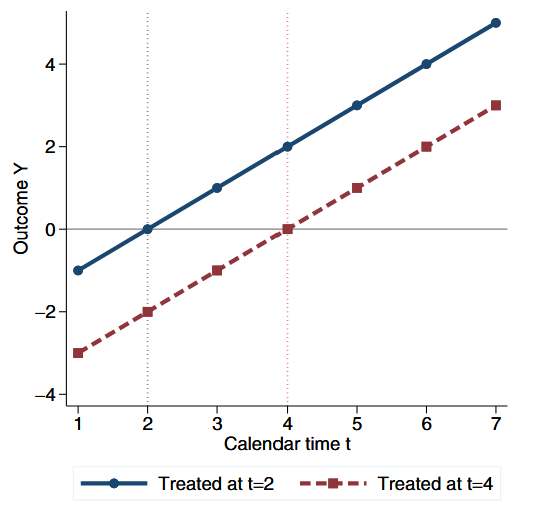
\includegraphics{borusyakRevisitingEventStudyDesigns2024_fig1.png}}
    \end{center}
    \medskip
    {\footnotesize Note: This figure shows the evolution of outcomes over seven periods for two units (or cohorts), for the illustrative example of Section 3.2. Vertical lines mark the periods in which the two units are first treated.}
    \label{borusyakRevisitingEventStudyDesigns2024_fig1}
\end{figure}

To illustrate this result with a simple example, Figure \ref{borusyakRevisitingEventStudyDesigns2024_fig1} plots the outcomes for a simulated dataset with two units, on treated at $t=2$ and the other at $t=4$. Both units exhibit linear growth in the outcome, starting from different levels. There are two interpretations of these dynamics. First, treatment could have no impact on the outcome, in which case the level difference corresponds to the unit FEs, while trends are just a common feature of the environment, through period FEs. Alternatively, note that the outcome equals the number of periods since the event for both groups and all time periods: it is zero at the moment of treatment, negative before, and positive after. A possible interpretation is that the outcome is entirely driven by causal effects and anticipation of treatment. Thus, one cannot hope to distinguish between unrestricted dynamic causal effects and a combination of unit effects and time trends. \footnote{Formally, the problem arises because a linear time trend $t$ and a linear term in the cohort $E_i$ (subsumed by the unit FEs) can perfectly reproduce a linear term in horizon $K_{it} = t - E_i$. Therefore, a complete set of treatment leads and lags, which is equivalent to the horizon FEs, is collinear with the unit and period FEs.}

The problem may be important in practice, as statistical packages may resolve this collinearity by dropping an arbitrary unit or period indicator. Some estimates of $\bc{\tau_h}$ would then be produced, but because of an arbitrary trend in the coefficients they may suggest a violation of parallel trends even when the specification is in fact correct, that is, Assumptions \ref{PT} and \ref{NA} hold and there is no heterogeneity of treatment effects for each horizon (Assumption \ref{RCE}).    

To break the collinearity problem, stronger restrictions on anticipation effects, and thus on $Y_{it}$ for untreated observations, have to be introduced. One could consider imposing minimal restrictions on the specification that would make it identified. In typical cases, only a linear trend in $\bc{\tau_h}$ is not identified in the fully dynamic specification, while non-linear paths cannot be reproduced with unit and period fixed effects. Therefore, just one additional normalization, for example, $\tau_{-a}=0$ in addition to $\tau_{-1}=0$, breaks multi-collinearity.

However, minimal identified models rely on ad hoc identification assumptions which are a priori unattractive. For instance, just imposing $\tau_{-a} = \tau_{-1} = 0$ means that anticipation effects are assumed away $1$ and $a$ periods before treatment, but not in other pre-periods. This assumption therefore depends on the realized event times. Instead, a systematic approach is to impose the assumptions -- some forms of no-anticipation effects and parallel trends -- that the researcher has an a priori argument for and which motivated the use of DiD. Such assumptions also give much stronger identification power. 

\subsection{Negative Weighting in the Static Regression}

We now show how, by imposing Assumption \ref{RCE} instead of specifying the estimation target, the static TWFE specification does not identify a reasonably weighted average of heterogeneous treatment effects: the underlying weights may be negative, particularly for the long-run causal effects. The issues we discuss here also arise in dynamic specifications that bin multiple lags together. 

First, we note that, if the parallel-trends and no-anticipation assumptions hold, the static specification identifies some weighted average of treatment effects.
\begin{proposition}
    If Assumptions \ref{PT} and \ref{NA} hold, then the estimand of the static specification in Equation (\ref{3}) satisfies $\tau^{\text{static}} = \sum_{it \in \O_1} \o_{it}^{\text{static}} \tau_{it}$ for some weights $\o_{it}^{\text{static}}$ that do not depend on the outcome realizations and add up to one, $\sum_{it \in \O_1} \o_{it}^{\text{static}} = 1$.
\end{proposition}

The underlying weights $\o_{it}^{\text{static}}$ can be computed from the data using the Frisch-Waugh-Lovell theorem and only depend on the timing of treatment for each unit and the set of observed units and periods. The static specification's estimand, however, cannot be interpreted as a proper weighted average, as some weights can be negative, which we illustrate with a simple example. 

\begin{proposition}
    Suppose Assumptions \ref{PT} and \ref{NA} hold and the data consists of two units, $A$ and $B$, treated in periods $2$ and $3$, respectively, both observed in periods $t=1,2,3$. Then the estimand of the static specification (\ref{3}) can be expressed as 
    $$
    \tau^{\text{static}} = \tau_{A2} + \frac{1}{2} \tau_{B3} - \frac{1}{2} \tau_{A3}.
    $$
\end{proposition}


\begin{figure}[H]
    \noindent\caption{Two-unit, three-period example}
    \begin{center}
        \resizebox{0.7\textwidth}{!}{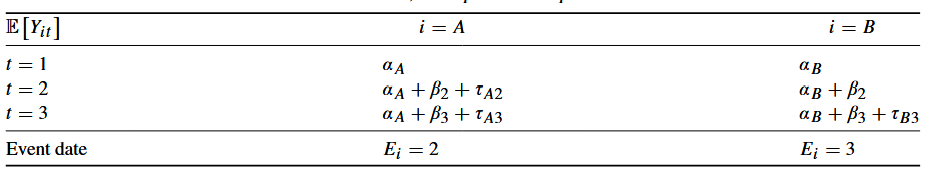
\includegraphics{borusyakRevisitingEventStudyDesigns2024_tab1.png}}
    \end{center}
    \medskip
    {\footnotesize This table shows the evolution of expected outcomes over three periods for two units (or cohorts), for the illustrative example of Proposition 3. Without loss of generality, we normalize $\b_1 = 0$.}
    \label{borusyakRevisitingEventStudyDesigns2024_tab1}
\end{figure}

This example illustrates the severe short-run bias of the static specification: the long-run causal effect, corresponding to the early treated unit $A$ and the late period $3$, enters with a negative weight ($-1/2$). Thus, larger long-run effects make the coefficient smaller.

This problem results from what we call ``forbidden comparisons'' performed by the static specification. Recall that the original idea of DiD estimation is to compare the evolution of outcomes over some time interval for the units which got treated during that interval relative to a reference group of units which didn't, identifying the period FEs. In the Proposition 3 example, such an ``admissible'' comparison is between units $A$ and $B$ in periods $2$ and $1$, $\bp{Y_{A2} - Y_{A1}} - \bp{Y_{B2} - Y_{B1}}$. However, panels with staggered treatment timing also lend themselves to a second type of comparisons, in which the reference group has been treated throughout the relevant period. For units in this group, the treatment indicator $D_{it}$ does not change over the relevant period, and so the restrictive specification uses them to identify period FEs, too. The comparison between units $B$ and $A$ in periods $3$ and $2$, $\bp{Y_{B3} - Y_{B2}} - \bp{Y_{A3} - Y_{A2}}$. While a comparison like this is appropriate and increases efficiency when treatment effects are homogeneous (which the static specification was designed for), forbidden comparisons are problematic under treatmenteffect heterogeneity.

For instance, subtracting $\bp{Y_{A3} - Y_{A2}}$ not only removes the gap in period FEs, $\b_3 - \b_2$, but also deducts the evolution of treatment effects $\tau_{A3} - \tau_{A2}$, placing a negative weight on $\tau_{A3}$. The restrictive specification leverages comparisons of both types.

Fundamentally, this problem arises because the specification imposes very strong restrictions on treatment-effect homogeneity, that is, Assumption \ref{RCE}, instead of acknowledging the heterogeneity and specifying a particular target estimand (or perhaps a class of estimands that the researcher is indifferent between).

With a large number of never-treated units or a large number of periods before any unit is treated (relative to other units and periods), our setting becomes closer to a classical nonstaggered DiD design, and therefore negative weights disappear, as our next result illustrates:

\begin{proposition}
    Suppose all units are observed for all periods $t = 1, \ldots, T$ and the earliest treatment happens at $E_{\text{first}}>1$. Let $N_1^*$ be the number of observations for never-treated units before period $E_{\text{first}}$ and $N_0^*$ be the number of untreated observations for ever-treated units since $E_{\text{fist}}$. Then there is no negative weighting, that is, $\min_{it \in \O_1} \o_{it}^{\text{static}} \geq 0$ if and only if $N_1^* \geq N_0^*$.
\end{proposition}

\subsection{Spurious Identification of Long-Run Effects in Dynamic Specifications}

Another consequence of inappropriately imposing Assumption \ref{RCE} concerns estimation of long-run causal effects. Conventional dynamic specifications (except those subject to the under-identification problem) yield some estimates for all $\tau_h$ coefficients. Yet, for large enough $h$, no averages of treatment effects are identified under Assumptions \ref{PT} and \ref{NA} with unrestricted treatment-effect heterogeneity. Therefore, estimates from restrictive specifications are fully driven by unwarranted extrapolation of treatment effects across observations and may not be reliable, unless strong ex ante reasons for Assumption \ref{RCE} exist.

The issue is well illustrated in the example of Proposition 3. To identify the long-run effect $\tau_{A3}$ under Assumptions \ref{PT} and \ref{NA}, one needs to form an admissible DiD comparison, of the outcome growth over some period between unit $A$ and another unit not yet treated in period $3$. However, by period $3$ both units have been treated. Mechanically, this problem arises because the period fixed effect $\b_3$ is not identified separately from the treatment effects $\tau_{A3}$ and $\tau_{B3}$ in this example, absent restrictions on treatment effects. Yet, the semi-dynamic specification 
\begin{equation}
    \notag 
    Y_{i t}=\tilde{\alpha}_i+\tilde{\beta}_t+\tau_0 \mathbf{1}\left[K_{i t}=0\right]+\tau_1 \mathbf{1}\left[K_{i t}=1\right]+\tilde{\varepsilon}_{i t}
\end{equation}
will produce an estimate $\wt{\tau}_1$ via extrapolation. Specifically, two different parameters, $\tau_{A3} - \tau_{B3}$ and $\tau_{A2}$, are identified by comparing the two units in periods $2$ or $3$, respectively, with period $1$. Therefore, when imposing homogeneity of short-run effects across units, $\tau_{A2} = \tau_{B3} = \tau_0$, we estimate the long-run effect $\tau_{A3} \equiv \tau_1$ as the sum of $\tau_1 - \tau_0$ and $\tau_0$:
\begin{equation}
    \notag 
    \hat{\tau}_1=\left[\left(Y_{A 3}-Y_{A 1}\right)-\left(Y_{B 3}-Y_{B 1}\right)\right]+\left[\left(Y_{A 2}-Y_{A 1}\right)-\left(Y_{B 2}-Y_{B 1}\right)\right] .
\end{equation}
However, when $\tau_{A2} \neq \tau_{B3}$, this estimator is biased. 

In general, the gap between the earliest and the latest event times observed in the data provides an upper bound on the number of dynamic coefficients that can be identified without extrapolation of treatment effects. This result, which follows by the same logic of non-identification of the later period effects, is formalized by our next proposition:

\begin{proposition}
    Suppose there are no never-treated units and let $\ol{H} = \max_i E_i - \min_i E_i$. Then, for any non-negative weights $\o_{it}$ defined over the set of observations with $K_{it} \geq \ol{H}$ (that are not identically zero), the weighted sum of causal effects $\sum_{it \in K_{it} \geq \ol{H}} \o_{it} \tau_{it}$ is not identified by Assumptions \ref{PT} and \ref{NA}.
\end{proposition}

\section{Imputation-Based Estimation and Testing}





\bibliography{\CiteReference}


\end{document}
